\subsection{Learning Rate}\label{sec:learningrate}
We have discussed the importance of parameters such as weights and biases, known as machine-learnable parameters. However, the learning rate $\eta$ is a configurable hyper-parameter\footnote{Hyper-parameter is a parameter used to control the learning process. } used in the training of neural networks. Unlike machine-learnable parameters, which are derived from the learning process, the learning rate must be predefined to tweak the model's output as well as to monitor how the algorithms learn.
%Evidently by Fig. \ref{fig:multilearn}, the learning rate is significant. 

\begin{figh}
        \begin{subfigure}[h]{0.48\linewidth}
    \centering
    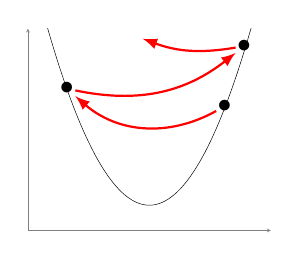
\begin{tikzpicture}[scale=.45]
        \begin{axis}[   
            grid=minor,  
            ticks=none,
            xmin=0,
            xmax=4,
            axis x line=middle,
            ymax=.8,
            ymin=0,
            axis y line=left,
            no markers,
            axis line style=gray,
            xlabel style=gray,
            ylabel style=gray,
        ]
            \addplot[black,mark=none,samples=200,domain=0:10,] (x,{(x/2-1)^2+.1});
            %\addplot[dashed,black,mark=none,samples=200,domain=0:10,] (x,{.7*x-1.8});
        \end{axis}
        
        \node[inner sep=1mm] (A) at (5.55,3.5){};
        \node[inner sep=1mm] (B) at (1.1,4){};
        \node[inner sep=1mm] (C) at (6.1,5.2){};
        \node[inner sep=1mm] (D) at (3,5.5){};
        
        \draw[-latex,red, thick] (A) edge[bend left=35] (B);
        \draw[-latex,red, thick] (B) edge[bend right=25] (C);
        \draw[-latex,red, thick] (C) edge[bend left=15] (D);
        
        \node[inner sep=-.2mm] at (A){$\bullet$};
        \node[inner sep=-.2mm] at (B){$\bullet$};
        \node[inner sep=-.2mm] at (C){$\bullet$};
\end{tikzpicture}
    \caption{}
    \label{fig:learnveryhigh}
\end{subfigure}
\hfill
\begin{subfigure}[h]{0.48\linewidth}
    \centering
    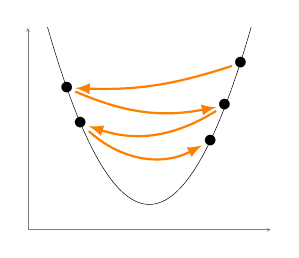
\begin{tikzpicture}[scale=.45]
        \begin{axis}[   
            grid=minor,  
            ticks=none,
            xmin=0,
            xmax=4,
            axis x line=middle,
            ymax=.8,
            ymin=0,
            axis y line=left,
            no markers,
            axis line style=gray,
            xlabel style=gray,
            ylabel style=gray
        ]
            \addplot[black,mark=none,samples=200,domain=0:10,] (x,{(x/2-1)^2+.1});
            %\addplot[dashed,black,mark=none,samples=200,domain=0:10,] (x,{.7*x-1.8});
        \end{axis}
        
        \node[inner sep=1mm] (A) at (6,4.7){};
        \node[inner sep=1mm] (B) at (1.1,4){};
        \node[inner sep=1mm] (C) at (5.55,3.5){};
        \node[inner sep=1mm] (D) at (1.48,3){};
        \node[inner sep=1mm] (E) at (5.15,2.5){};
        
        \draw[-latex,orange, thick] (A) edge[bend left=10] (B);
        \draw[-latex,orange, thick] (B) edge[bend right=17] (C);
        \draw[-latex,orange, thick] (C) edge[bend left=25] (D);
        \draw[-latex,orange, thick] (D) edge[bend right=35] (E);
        
        \node[inner sep=-.2mm] at (A){$\bullet$};
        \node[inner sep=-.2mm] at (B){$\bullet$};
        \node[inner sep=-.2mm] at (C){$\bullet$};
        \node[inner sep=-.2mm] at (D){$\bullet$};
        \node[inner sep=-.2mm] at (E){$\bullet$};
\end{tikzpicture}
    \caption{}
    \label{fig:learnhigh}
\end{subfigure}
\vspace{2mm}
\begin{subfigure}[h]{0.48\linewidth}
    \centering
    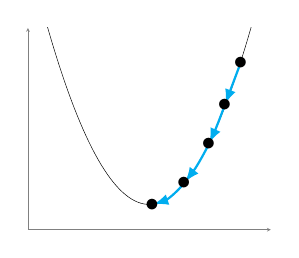
\begin{tikzpicture}[scale=.45]
        \begin{axis}[   
            grid=minor,  
            ticks=none,
            xmin=0,
            xmax=4,
            axis x line=bottom,
            ymax=.8,
            ymin=0,
            axis y line=left,
            no markers,
            axis line style=gray,
            xlabel style=gray,
            ylabel style=gray
        ]
            \addplot[black,mark=none,samples=200,domain=0:10,] (x,{(x/2-1)^2+.1});
            %\addplot[dashed,black,mark=none,samples=200,domain=0:10,] (x,{.7*x-1.8});
        \end{axis}
        
        \node[inner sep=-.2mm] (A) at (6,4.7){};
        \node[inner sep=-.2mm] (B) at (5.55,3.5){};
        \node[inner sep=-.2mm] (C) at (5.1,2.4){};
        \node[inner sep=-.2mm] (D) at (4.4,1.3){};
        \node[inner sep=-.2mm] (E) at (3.5,.7){};
        
        \draw[-latex,cyan, thick] (A) -- (B);
        \draw[-latex,cyan, thick] (B) edge[bend left=2] (C);
        \draw[-latex,cyan, thick] (C) edge[bend left=5] (D);
        \draw[-latex,cyan, thick] (D) edge[bend left=15] (E);
        
        \node[inner sep=-.2mm] at (A){$\bullet$};
        \node[inner sep=-.2mm] at (B){$\bullet$};
        \node[inner sep=-.2mm] at (C){$\bullet$};
        \node[inner sep=-.2mm] at (D){$\bullet$};
        \node[inner sep=-.2mm] at (E){$\bullet$};
        
	\end{tikzpicture}
    \caption{}
    \label{fig:learnopt}
\end{subfigure}
\hfill
\begin{subfigure}[h]{0.48\linewidth}
    \centering
    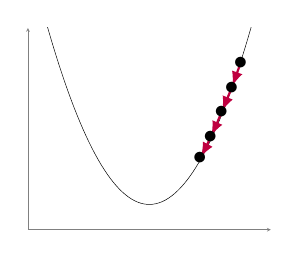
\begin{tikzpicture}[scale=.45]
        \begin{axis}[   
            grid=minor,  
            ticks=none,
            xmin=0,
            xmax=4,
            axis x line=bottom,
            ymax=.8,
            ymin=0,
            axis y line=left,
            no markers,
            axis line style=gray,
            xlabel style=gray,
            ylabel style=gray
        ]
            \addplot[black,mark=none,samples=200,domain=0:10,] (x,{(x/2-1)^2+.1});
            %\addplot[dashed,black,mark=none,samples=200,domain=0:10,] (x,{.7*x-1.8});
        \end{axis}
        
        \node[inner sep=-.2mm] (A) at (6,4.7){};
        \node[inner sep=-.2mm] (B) at (5.75,4){};
        \node[inner sep=-.2mm] (C) at (5.46,3.3){};
        \node[inner sep=-.2mm] (D) at (5.15,2.6){};
        \node[inner sep=-.2mm] (E) at (4.85,2){};
        
        \draw[-latex,purple, thick] (A) -- (B);
        \draw[-latex,purple, thick] (B) -- (C);
        \draw[-latex,purple, thick] (C) edge[bend left=1] (D);
        \draw[-latex,purple, thick] (D) edge[bend left=2] (E);
        
        \node[inner sep=-.2mm] at (A){$\bullet$};
        \node[inner sep=-.2mm] at (B){$\bullet$};
        \node[inner sep=-.2mm] at (C){$\bullet$};
        \node[inner sep=-.2mm] at (D){$\bullet$};
        \node[inner sep=-.2mm] at (E){$\bullet$};
        
	\end{tikzpicture}
    \caption{}
    \label{fig:learnlow}
\end{subfigure}
        \caption{(a) Very high $\eta$ causes divergences (b) High $\eta$ causes overshooting (c) Optimal $\eta$ converges to minima (d)  Low $\eta$ converges slowly towards minima.}
        \label{fig:multilearn}
\end{figh}
    
As like the activation and cost functions, the learning rate is given by a function of preference.  \textcite{wu2019demystifying} states choosing an appropriate learning rate can be difficult, as depicted in \autoref{fig:multilearn}.
As if $\eta$ is small, then due to the minor changes made to the weights of each update the rate of convergence will be slow, whence require more training epochs (one cycle through the full training dataset). In contrast, if $\eta$ is large, then due to rapid changes, the risk of overshooting arises but require fewer training epochs. In some cases this may lead to the variables diverging from the optimal and in others result in sub-optimality. Hence any desirable learning rate must have such trade offs.
    
The constant learning rate is a baseline default function for neural network frameworks (e.g.  Caffe)\footnote{Caffe is an open source deep learning framework originally developed at University of California, Berkeley.}. An optimum constant learning rate for a model cannot be calculated with analysis methods on a given dataset, however, a good sufficient learning rate can be achieved by trial and error \parencite{wu2019demystifying}.  In general, a popular and naive starting point is taking a relatively very small constant learning rate, for instance $\eta := 1\mathrm{e}{-1} = 0.1$. Then, decrement the exponential per simulation of the neural network until a suitable learning rate is produced, e.g. $1\mathrm{e}{-2}= 0.01$, $1\mathrm{e}{-3}= 0.001$, etc. 
%But of course alternative functions can be used instead of the default, for example, the fixed step size (decaying) learning rate. 

\subsection{Limitations of Gradient Descent}
While gradient descent has been shown to be very useful for achieving the objective function, there are indeed limitations:

\begin{itemize}[leftmargin=*]
    \item As previously stated, a suitable learning rate must be chosen to ensure the success of a parameter update policy. 
    \item If the error cost function has a large number of local minima, there is no guarantee that the process will find the global minimum \parencite{298667}.
    The gradient descent algorithm, in particular, does not distinguish between local and global minima, because once a process reaches a minima, it is unable to escape (given that the learning rate is not sufficiently large enough to exceed the size of the ditch). 
    \item The optimal parameters the process yields is dependable on the initialisation of the parameters, that is, let $\Bar{\theta}$ and $\Tilde{\theta}$ be distinct parameter initialisations, then $\Bar{\theta}^{[t^*]}$ and $\Tilde{\theta}^{[t^*]}$ may or may not be identical. This difference between the two optimal parameters the process yields can be as small as the $\epsilon$ in \cref{alg:grad} or can be a consequence of the limitation above, the parameters have converged into different minima.
\end{itemize}
